\section{敏感性、稳健性与一致性检验}
\subsection{时间标签敏感性}
将问题一的144点净负荷与电价整体平移$-10$、0、$+10$分钟并重新优化，费用分别为35,129.73、35,126.95和35,126.85元；相对主口径最大偏差仅2.78元，说明总费用对这一行序歧义不敏感。指定时段的解释仍应遵循官方模板行序。
\subsection{可行性与数值残差}
求解前以零储能、直接购电构造可行基线；求解后独立回代供需、SOC、容量边界及费用分量。问题二、问题4-2及两类价格下8种更新组合共6,570项检查全部通过，通过率100\%；所有SOC均位于$[1200,10800]$ kWh，误差处于浮点求解容差内。
\subsection{结果稳健性边界}
问题一将充放电效率从0.80提高到1.00后重新求解，费用曲线见相应记录，验证效率改善会单调扩大套利空间。问题三与问题4-3已穷举0/6/12/18构成的8种发布组合，均由不调整取得最低费用，结论并非仅来自两个端点。完整场景CVaR和不同调整结算解释仍应作为后续扩展。
\begin{figure}[H]\centering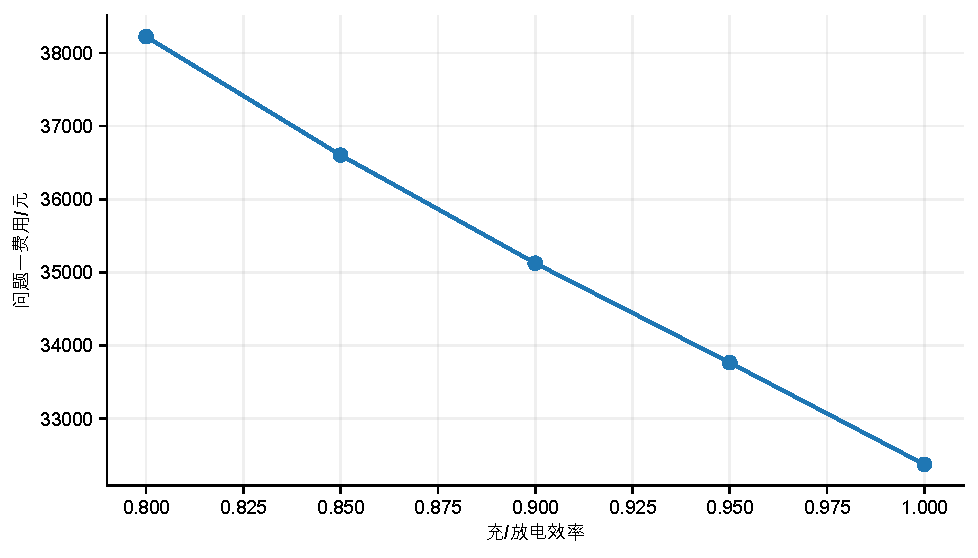
\includegraphics[width=0.78\textwidth]{../figures/fig08_efficiency_sensitivity.pdf}
\caption{问题一购电费用对储能充放电效率的敏感性}\label{fig:efficiency}\end{figure}
